	\appendix
	\section{Verilog}\label{sec:verilog}

		\subsection{Loop Filter and Reset Logic} \label{sec:lf_verilog}

	\begin{lstlisting}[language={Verilog}, caption={Loop filter hardware description.}, label={sim_code2}]
module lf
(
	input in, clk, rst, set_out, lf_en,
	input signed [13:0] b0, b1,
	input [12:0] init_out,
	output reg vco_rst, dac_rst,
	output [12:0] lf_out, lf_out_n
);
	reg last, wait_cycle1, wait_cycle2;
	reg signed [23:0] accum_reg;	// Output accumulator
	wire signed [13:0] p0, p1;		// PI filter products
	wire signed [23:0] sum;				// Accumulator sum
	reg [12:0] lf_rounded;				// Rounded integer portion
																// of accumulator for output

	// Muxes - Implements PI filter multipliers with a BBPD
	assign p0 = in ? b0 : ~b0 + 1; 
	assign p1 = last ? b1 : ~b1 + 1;

	// Accumulator sum
	assign sum = p0 + p1 + accum_reg;

	// Accumulator fractional part msb for output rounding decision
	assign frac_msb = sum[7];

	// set outputs OR'd with DAC reset as needed by CDACs
	assign lf_out = lf_rounded|{13{dac_rst}};
	assign lf_out_n = (~lf_rounded)|{13{dac_rst}};

	always @ (posedge clk) begin
    if (rst) begin 	// RST cycle 1: DCO+DAC RST
			dac_rst <= 1; 	// Assert DCO/DAC rst synchronously
			vco_rst <= 1; 
		end
		else if ((!rst)&&(dac_rst)) begin  
			dac_rst <= 0;		// RST Cycle 2: de-assert dac_rst,		
			wait_cycle1 <= 1;
		end
		else if (wait_cycle1) begin
			vco_rst <= 0;			// RST cycle 3: Wait 1 cycle
			wait_cycle1 <= 0;	// before BBPD sampling, no lf update
			wait_cycle2 <= 1;		
		end
		else if (wait_cycle2) begin
			wait_cycle2 <= 0;	// RST cycle 4: Wait 1 cycle
			last <= in;				// Record initial BBPD sample, no lf update
		end
		else if (lf_en) begin 	// Normal operation
			last <= in;
			accum_reg <= sum;
			lf_rounded <= frac_msb ? sum[20:8] + 1 : sum[20:8]; //output rounding
		end
		if (set_out) begin 	// Set output if set_out asserted
			accum_reg[23:21] <= {3{1'b0}};
			accum_reg[20:8] <= init_out[12:0];
			accum_reg[7:0] <= {8{1'b0}};
			lf_rounded <= init_out[12:0];	
		end
	end

endmodule
	    \end{lstlisting}

{\color{white}.}
\FloatBarrier\pagebreak

	\section{Layout}
		\subsection{Full Layout}\label{sec:full_lay}
			\begin{figure}[htb!]
			        \centering
			        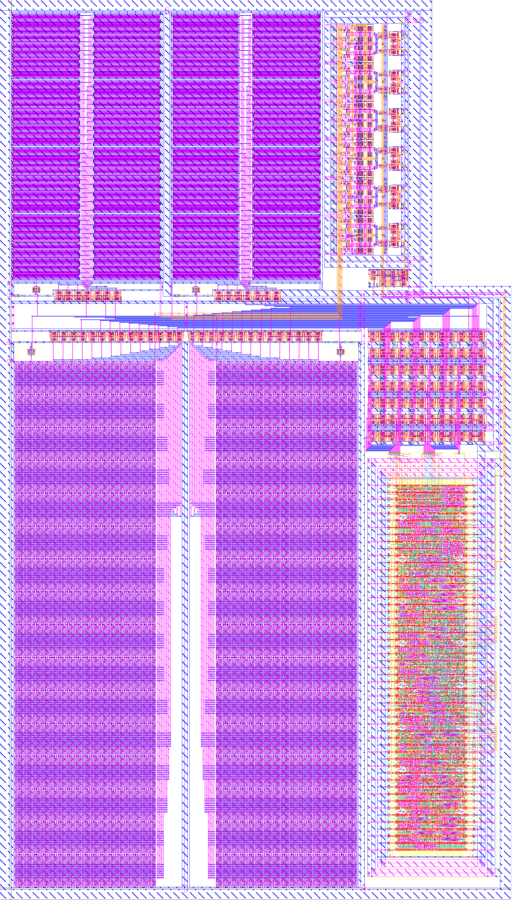
\includegraphics[height=0.8\textheight, angle=0]{./figs/layout/full_lay_1200dpi}
			    \caption{Full PLL Layout.}
			\end{figure}	
		{\color{white}.}
		\FloatBarrier\pagebreak	

		\subsection{Ring Oscillator}\label{sec:lay_osc}
				\begin{figure}[htb!]
				        \centering
				        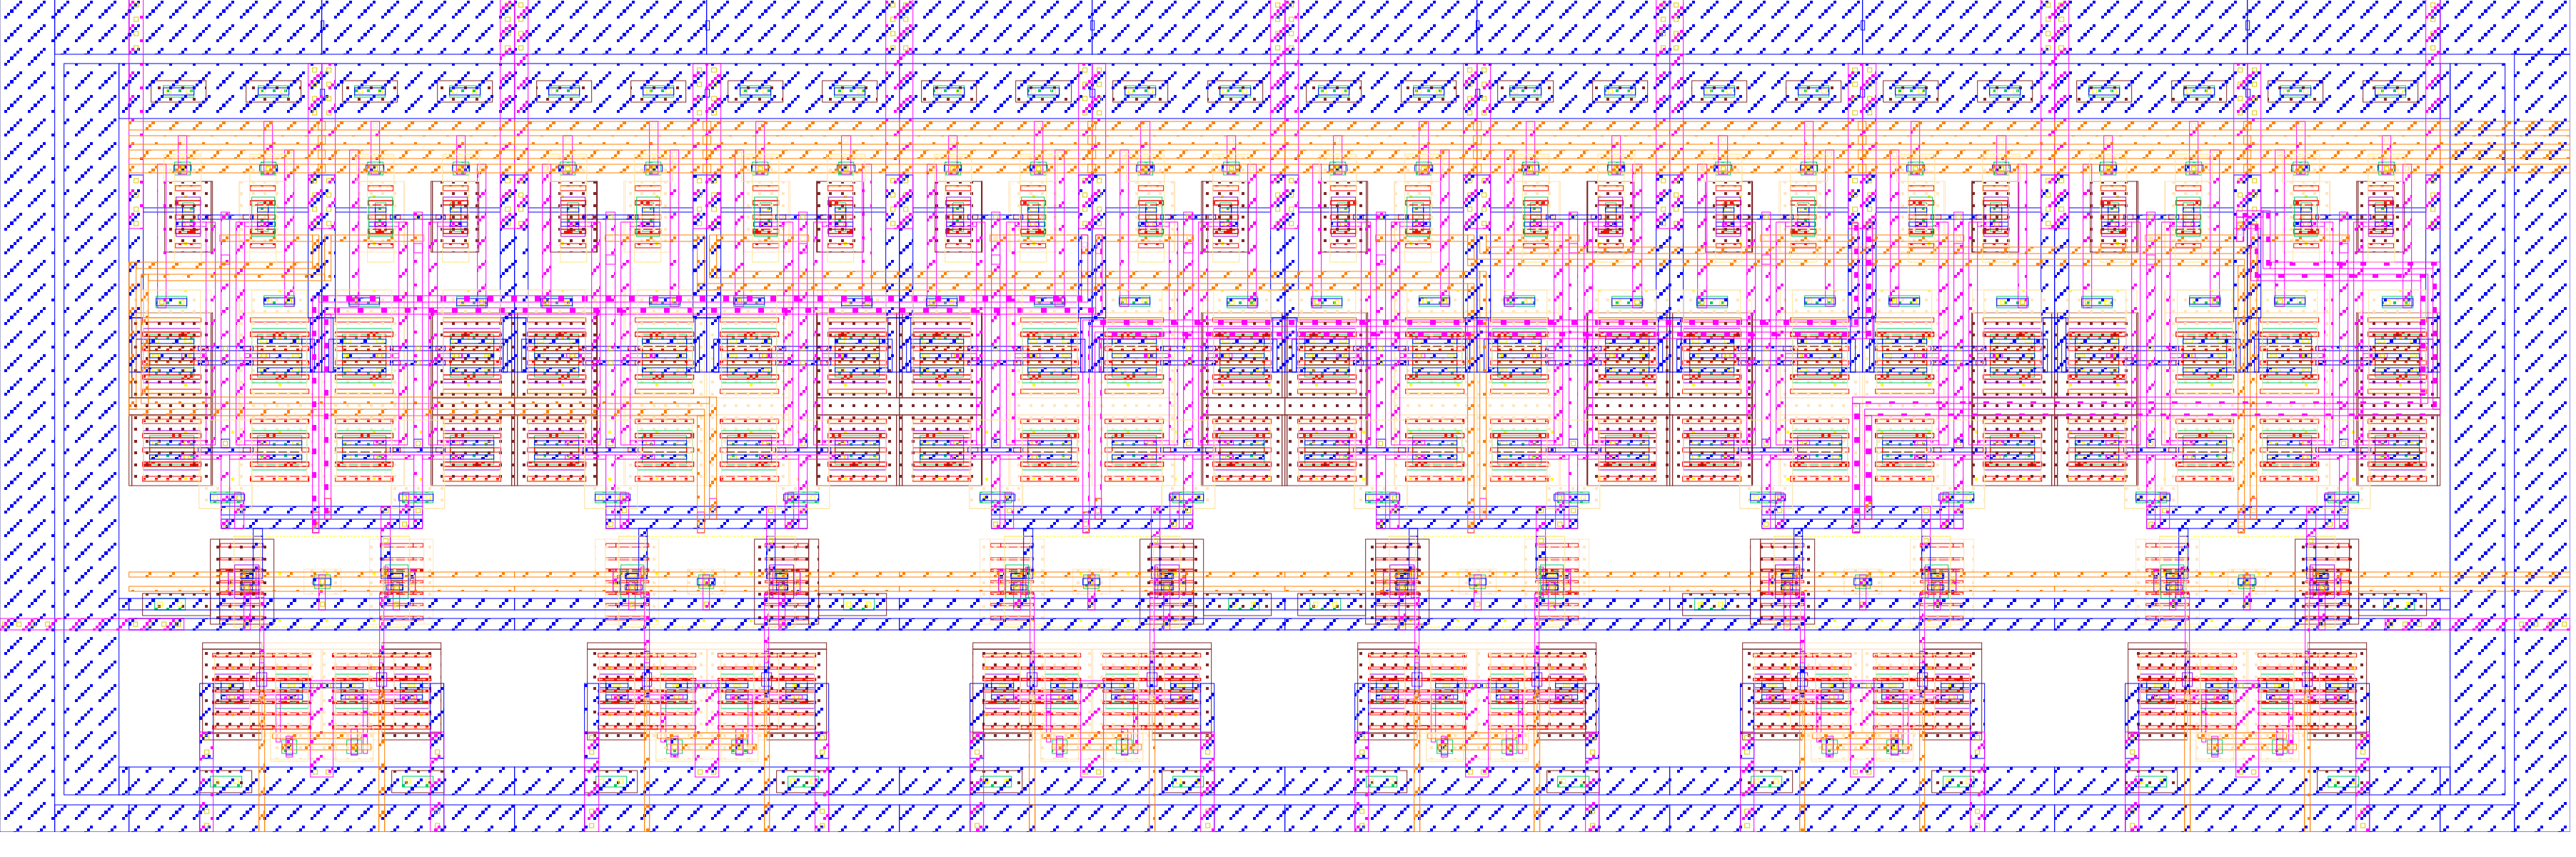
\includegraphics[height=0.75\textheight, angle=0]{./figs/layout/full_ro}
				    \caption{Full six stage oscillator layout with capacitor tuning bank, reset switches, and output buffer.}
				\end{figure}
			\FloatBarrier\pagebreak
			\subsubsection{Pseudodifferential Inverter Delay Cell}
				\begin{figure}[htb!]
				        \centering
				        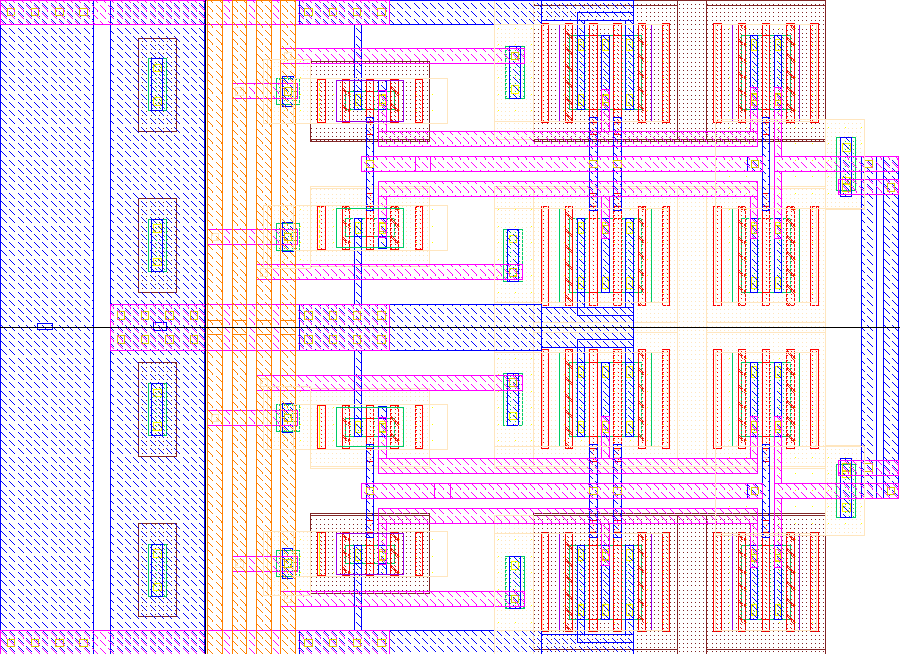
\includegraphics[width=0.8\textwidth, angle=0]{./figs/layout/dly_cell}
				    \caption{Unit delay stage pseudodifferential inverter.}
				\end{figure}
			\subsubsection{Reset Switches}
				\begin{figure}[htb!]
				        \centering
				        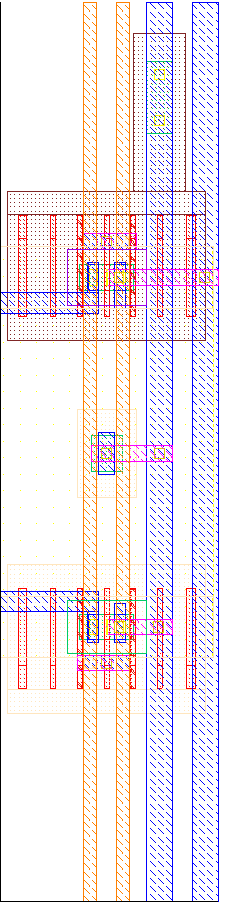
\includegraphics[height=0.4\textheight, angle=0]{./figs/layout/ro_sw}
				    \caption{Oscillator reset switches.}
				\end{figure}
			\subsubsection{Output Buffer}\label{sec:lay_buff}
				\begin{figure}[htb!]
				        \centering
				        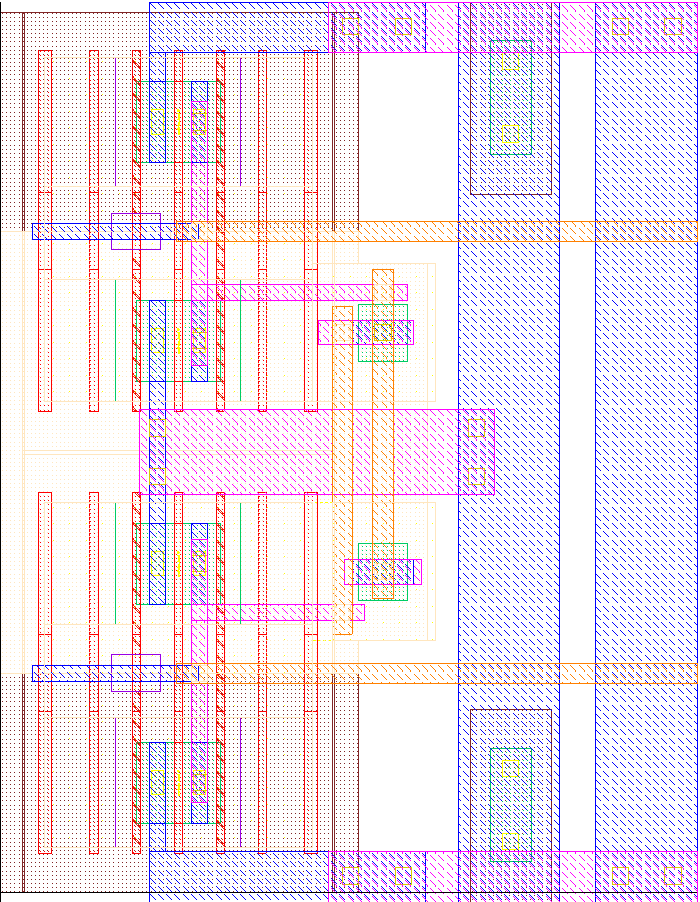
\includegraphics[height=0.4\textheight, angle=0]{./figs/layout/buffer}
				    \caption{Pseudodifferential inverter buffer cell.}
				\end{figure}
			% \FloatBarrier
			% \subsubsection{Capaitor tuning bank}
			% 	\begin{figure}[htb!]
			% 	        \centering
			% 	        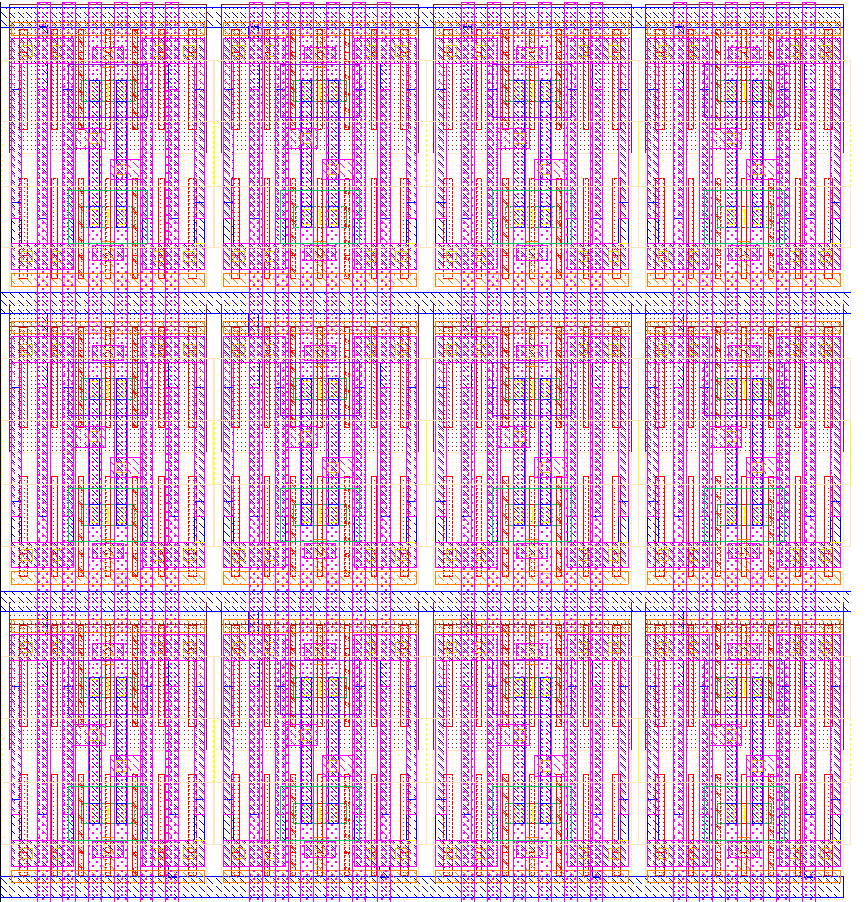
\includegraphics[width=0.6\textwidth, angle=0]{./figs/layout/layout_pvt_bank}
			% 	    \caption{Capaitor tuning bank.}
			% 	\end{figure}
		\FloatBarrier\pagebreak
		\subsection{10b CDAC}\label{sec:lay_cdac_10b}
			\subsubsection{Full CDAC Layout}
				\begin{figure}[htb!]
				        \centering
				        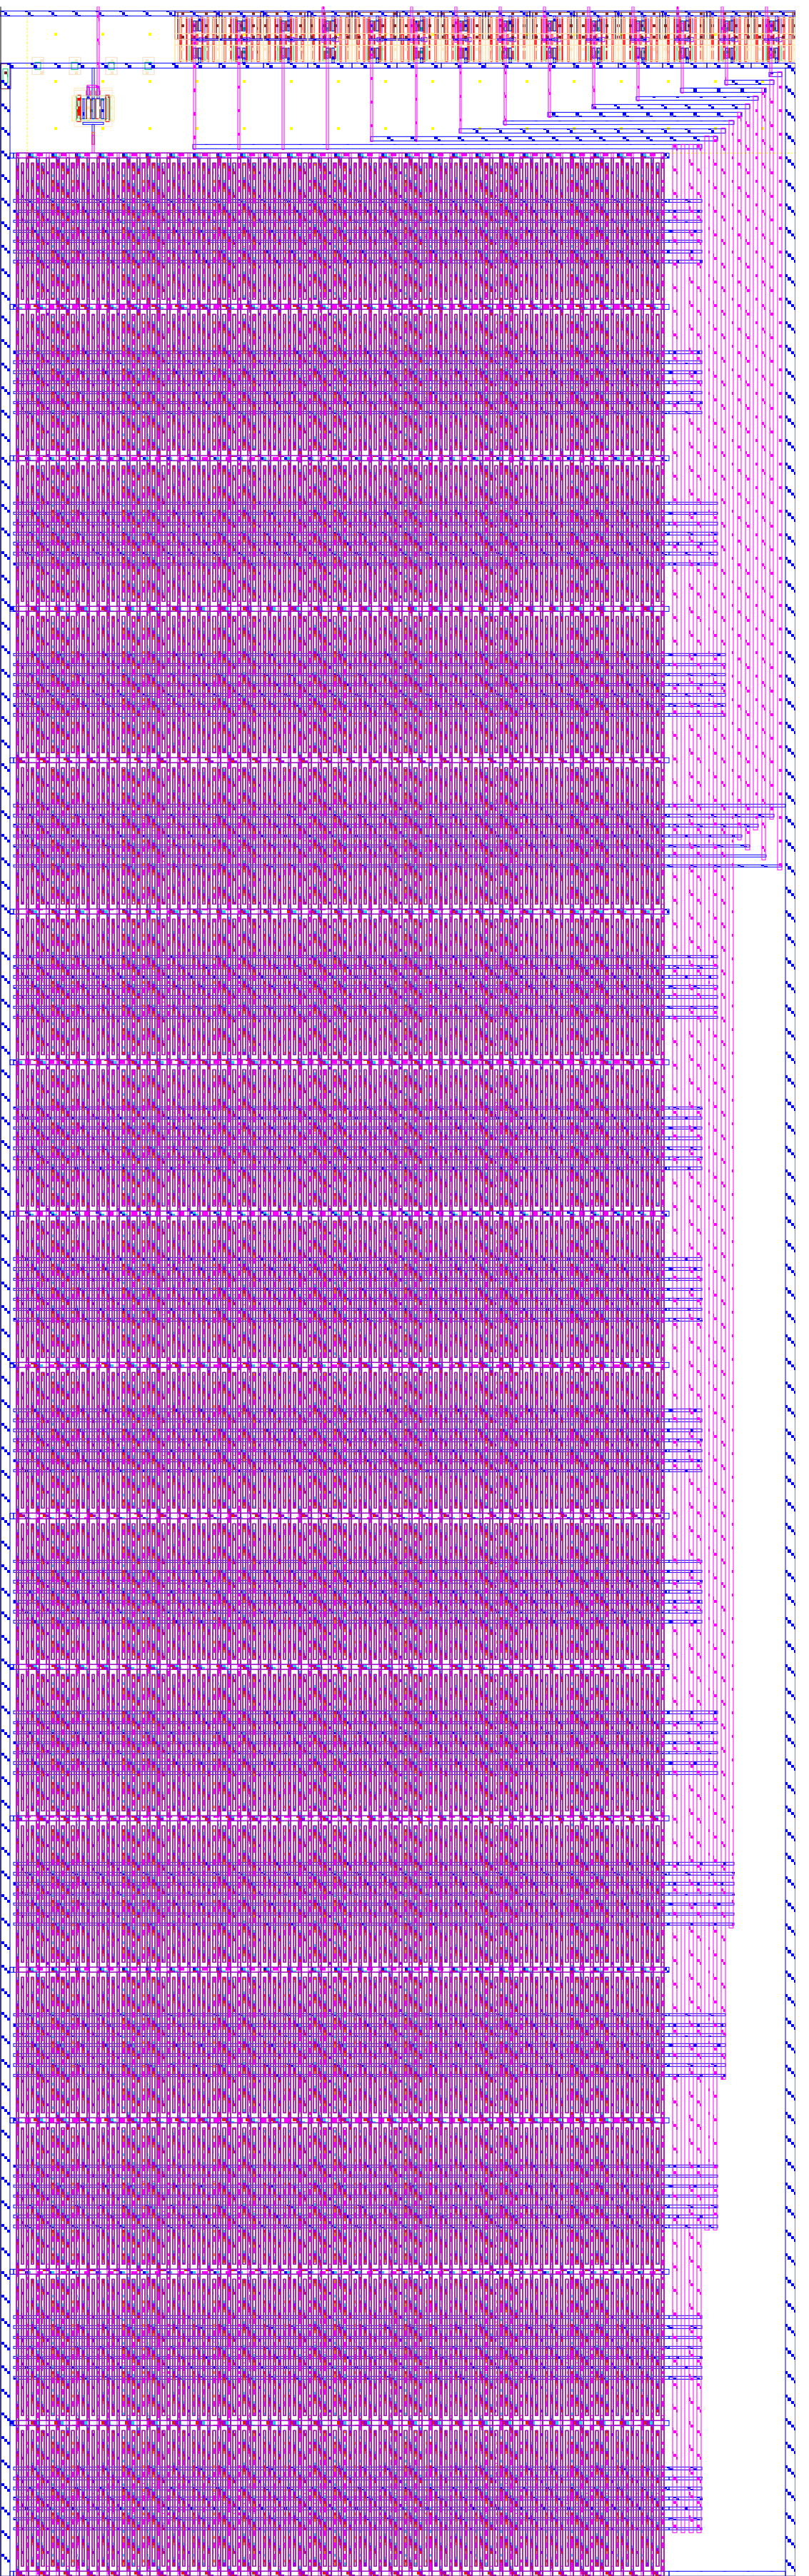
\includegraphics[height=0.85\textheight, angle=0]{./figs/layout/layout_cdac_10b}
				    \caption{10 bit CDAC layout.}
				\end{figure}
			\FloatBarrier\pagebreak
			\subsubsection{64 Unit Capacitor Sub-bank}
				\begin{figure}[htb!]
				        \centering
				        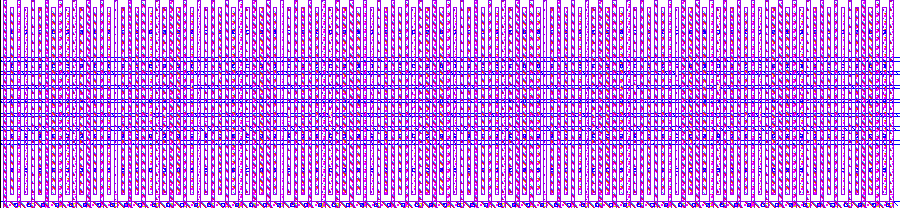
\includegraphics[width=\textwidth, angle=0]{./figs/layout/layout_cdac_unit_capbank}
				    \caption{64 unit capacitor bank.}
				\end{figure}
			\FloatBarrier
			\subsection{CDAC Capacitor Switch}
				\begin{figure}[htb!]
				        \centering
				        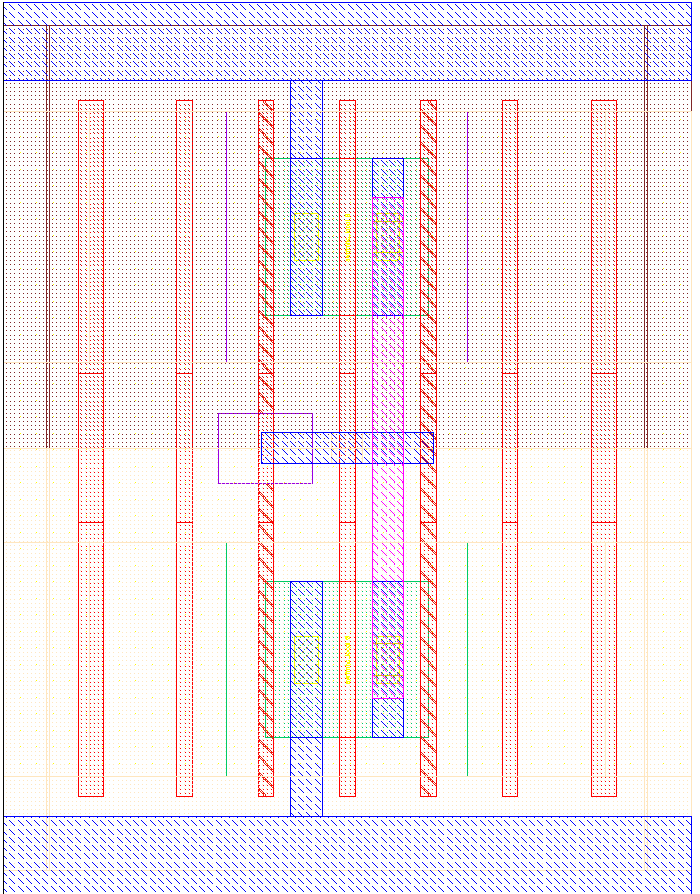
\includegraphics[width=0.5\textwidth, angle=0]{./figs/layout/layout_cdac_sw}
				    \caption{CDAC capacitor switch.}
				\end{figure}
		\FloatBarrier\pagebreak
		\subsection{3b CDAC}\label{sec:lay_cdac_3b}
			\begin{figure}[htb!]
			        \centering
			        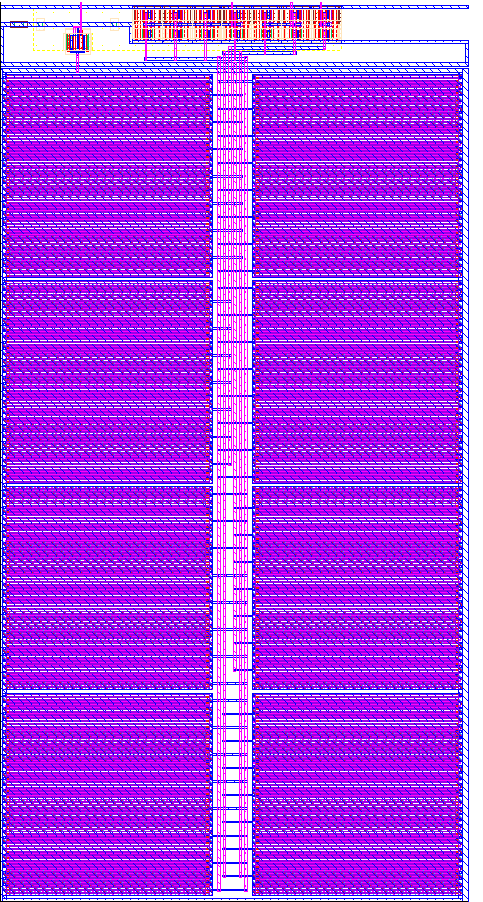
\includegraphics[height=0.85\textheight, angle=0]{./figs/layout/layout_cdac_3b}
			    \caption{3 bit CDAC layout.}
			\end{figure}
		\FloatBarrier\pagebreak
		% \subsection{Buffer}\label{sec:lay_buff}
		% 	\begin{figure}[htb!]
		% 	        \centering
		% 	        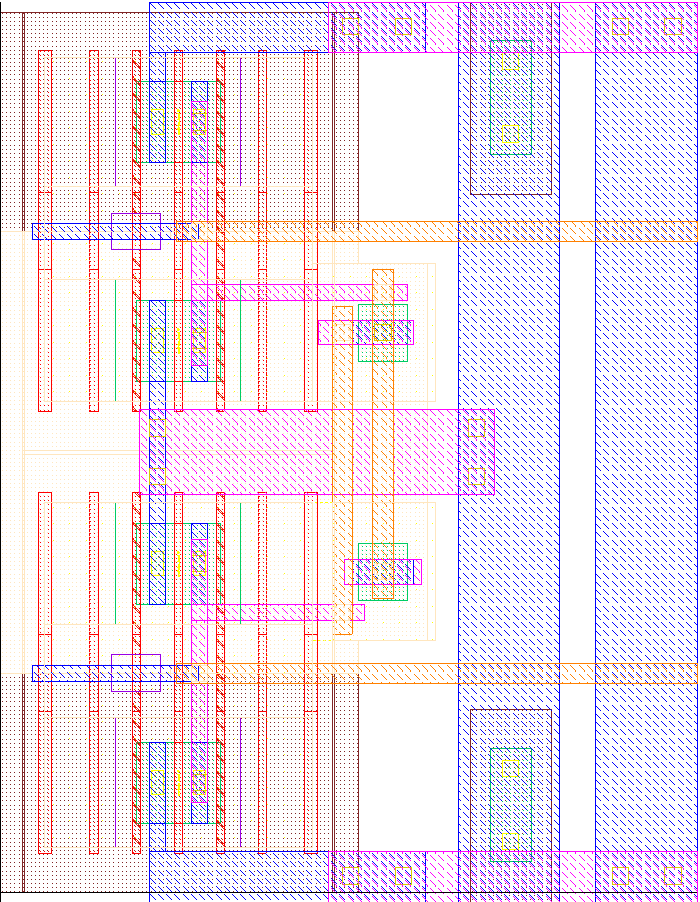
\includegraphics[width=0.8\textwidth, angle=0]{./figs/layout/buffer}
		% 	    \caption{Pseudodifferential inverter buffer cell.}
		% 	\end{figure}
		% \FloatBarrier\pagebreak
		\subsection{BBPD}\label{sec:lay_bbpd}
			\begin{figure}[htb!]
			        \centering
			        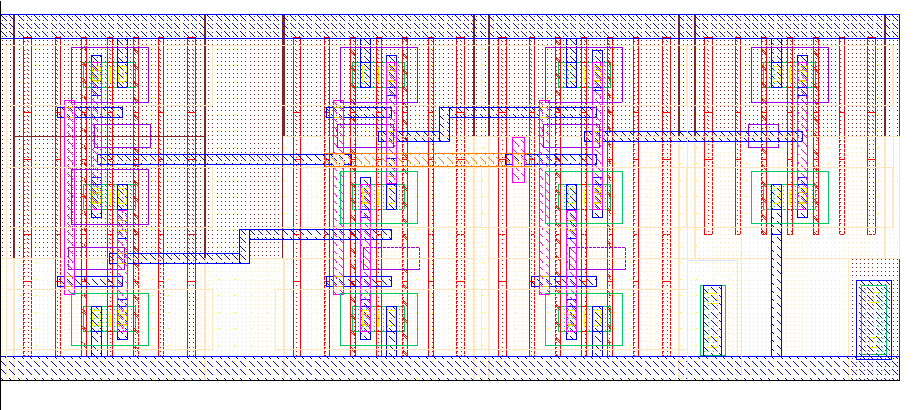
\includegraphics[width=\textwidth, angle=0]{./figs/layout/layout_bbpd}
			    \caption{Single ended bang-bang phase detector.}
			\end{figure}
		\subsection{Level Shifter}\label{sec:lay_ls}
			\begin{figure}[htb!]
			        \centering
			        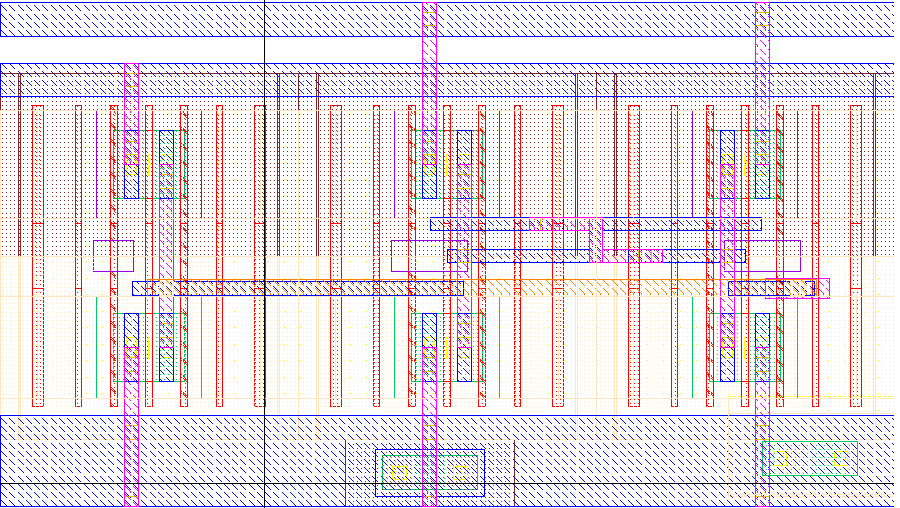
\includegraphics[width=\textwidth, angle=0]{./figs/layout/ls}
			    \caption{Low to high voltage domain level shifter.}
			\end{figure}
		\FloatBarrier\pagebreak
		\subsection{Loop Filter Logic}
			\begin{figure}[htb!]
			        \centering
			        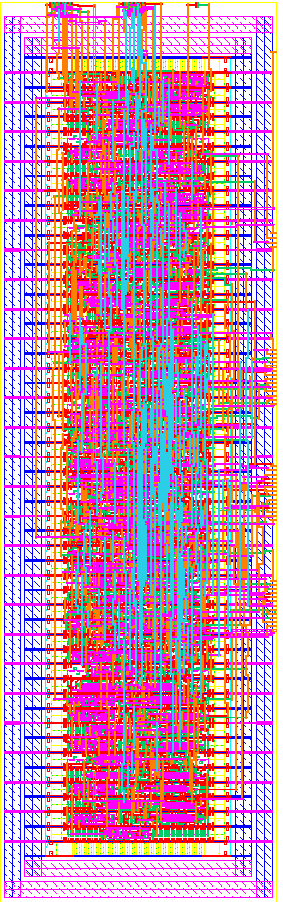
\includegraphics[height=0.8\textheight, angle=0]{./figs/layout/final_logic}
			    \caption{Place and route generated loop filter logic for PLL.}
			\end{figure}
		\FloatBarrier\pagebreak

\section{Extracted FD-SOI Device Parameters}\label{sec:fet_extracted_data}
		To analyze the body effect with FD-SOI backgates of the 22nm process technology used in this work, SPICE simulations to extract the body effect coefficient $\gamma$ and threshold voltage $V_{TH}$ for different channel lengths and bias conditions have been performed. Parameters for threshold voltage, and transconductances $g_m$ and $g_{mb}$ have been extracted using DC operating point simulations. Noting the relation from equation \ref{eq:gm_gmb_relation}, where $g_{mb} = \gamma g_{m}$, $\gamma$ can be deduced from operating point $g_m$ and $g_{mb}$ values. Figures \ref{fig:vth_vs_vbs} and \ref{fig:vth_slope_vs_vbs} show the extracted threshold voltage versus backgate bias and the slope of that relationship. Figures \ref{fig:vth_vs_len} and \ref{fig:gamma_vs_len} show the extracted threshold voltage and body effect coefficient versus channel length. Furthermore, table \ref{tab:nfet_vth_gamma} provides a selection of extracted N-channel device parameters, and table \ref{tab:pfet_vth_gamma} provides extracted P-channel devices parameters.

		It is observed that the threshold voltage slopes of figure \ref{fig:vth_groupa} are not perfectly linear, but for the simplified analytical purposes of this work, they can be approximated as linear. The P-channel devices in the technology of this work show a high degree of linearity, whereas the N-channel devices show variation in slope as in figure \ref{fig:vth_slope_vs_vbs}. It is also observed that the threshold voltage and body effect coefficient vary as channel lengths approach zero, but flatten out for longer device length. A final note is there is substantial variation of $\gamma$ and $V_{TH}$ between device types, so prudent care must be taken in the oscillator for selection of devices and their sizing.

		% \begin{equation}
		% V_{th} = V_{th0} - \gamma V_{BS}
		% \end{equation}

		\begin{figure}[htb!]
		    \centering
		    \begin{subfigure}{0.5\textwidth}
		        \centering
		        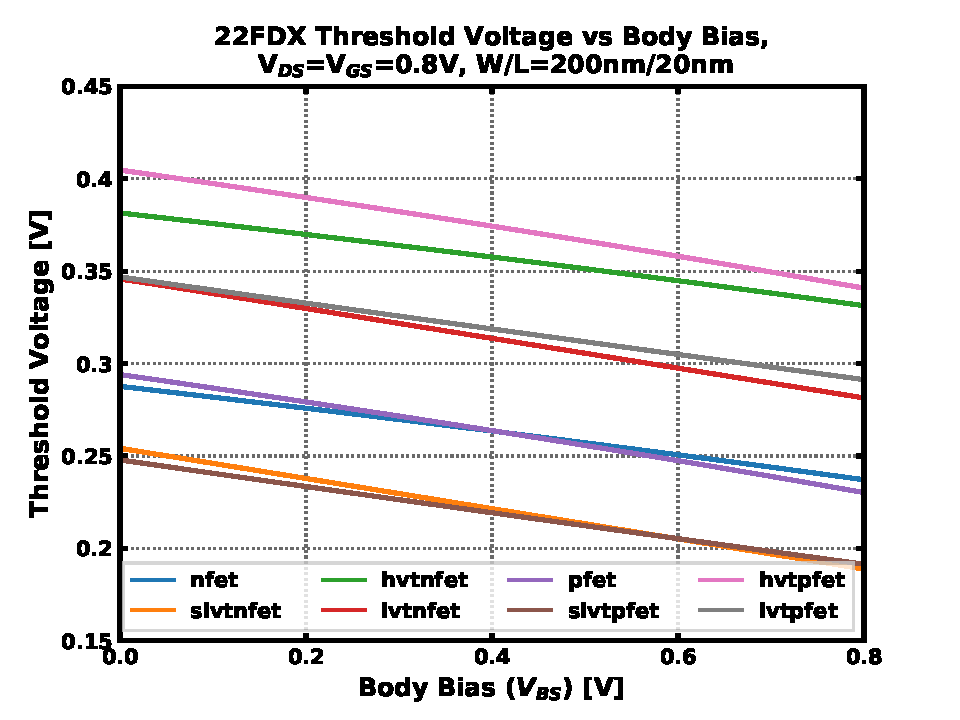
\includegraphics[width=1\textwidth, angle=0]{./figs/design/vth_vbs}
		        \caption{ }
		        \label{fig:vth_vs_vbs}
		    \end{subfigure}%
		    \begin{subfigure}{0.5\textwidth}
		        \centering
		        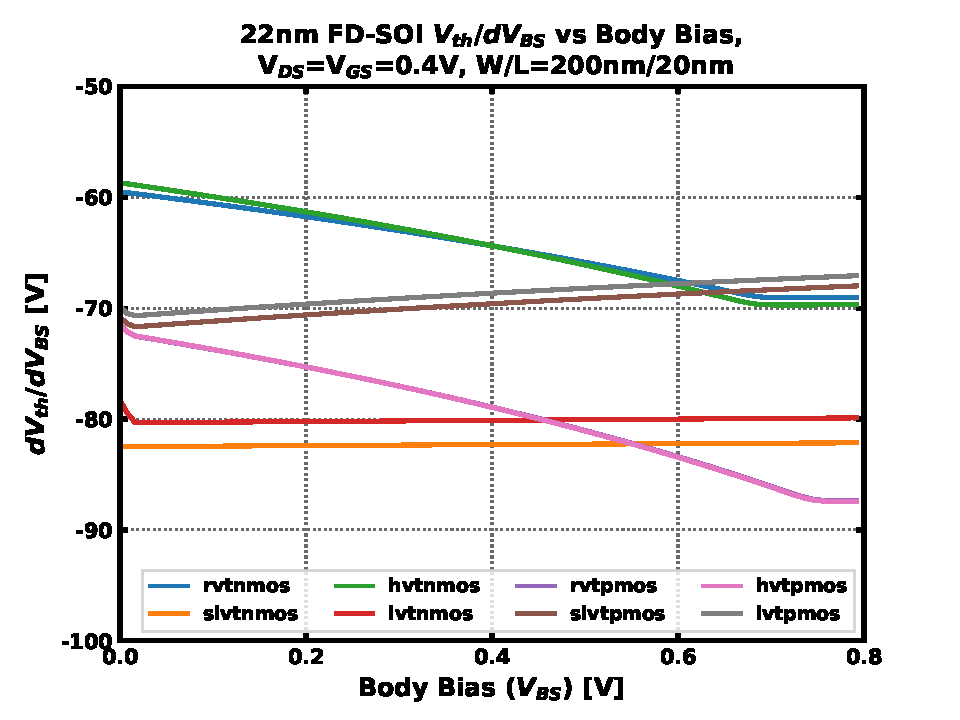
\includegraphics[width=1\textwidth, angle=0]{./figs/design/vth_slope_vbs}
		        \caption{ }
		        \label{fig:vth_slope_vs_vbs}
		    \end{subfigure}
		    % \caption{x.}
		    \caption{\textbf{(a)} 22nm FD-SOI process threshold voltage versus body bias, \textbf{(b)} Rate of change of threshold voltage versus body bias.}
		    \label{fig:vth_groupa}
		\end{figure} 


		\begin{figure}[htb!]
		    \centering
		    \begin{subfigure}{0.5\textwidth}
		        \centering
		        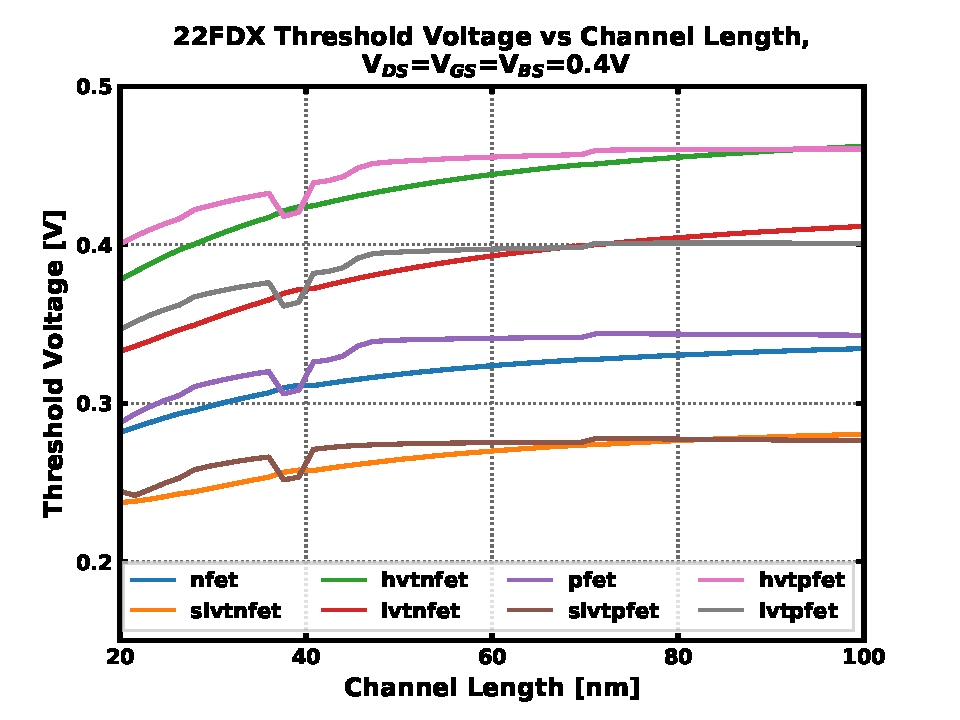
\includegraphics[width=1\textwidth, angle=0]{./figs/design/vth}
		        \caption{ }
		        \label{fig:vth_vs_len}
		    \end{subfigure}%
		    \begin{subfigure}{0.5\textwidth}
		        \centering
		        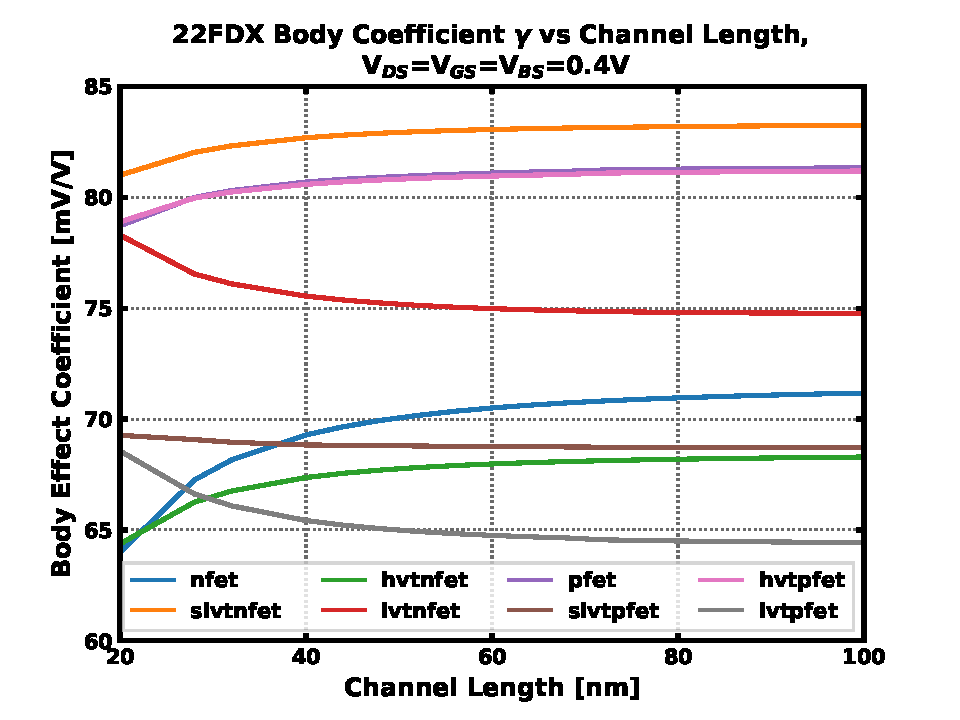
\includegraphics[width=1\textwidth, angle=0]{./figs/design/gamma}
		        \caption{ }
		        \label{fig:gamma_vs_len}
		    \end{subfigure}
		    % \caption{x.}
		    \label{fig:vth_groupb}
		    \caption{\textbf{(a)} 22nm FD-SOI process extracted threshold voltage versus channel length, \textbf{(b)} Extracted body effect coefficient.}
		\end{figure} 


\FloatBarrier


			\begin{table}[htb!]
				\centering
				\def\arraystretch{1.5}		
				\setlength\arrayrulewidth{1pt}
				\setlength{\tabcolsep}{1em} % for the horizontal padding
				\fontfamily{\sfdefault}\selectfont 
				\begin{tabular}{|l|l|l|l|l|}	
					\hline 
					\rule[-1ex]{0pt}{2.5ex} \cellcolor{gray!40}\textbf{Device} & \cellcolor{gray!40}\textbf{L [nm]} & \cellcolor{gray!40}\textbf{W [nm]} & \cellcolor{gray!40}\textbf{$V_{th}$ [mV]} & \cellcolor{gray!40}\textbf{$\gamma$ [mV/V]}\\ 
					\hline 
					\rule[-1ex]{0pt}{2.5ex} \textbf{rvtnmos} & 20 & 100 & 306.3 & 59.14 \\ 
					\hline 
					\rule[-1ex]{0pt}{2.5ex} \textbf{rvtnmos} & 100 & 500 & 376.4 & 65.4 \\ 
					\hline 
					\rule[-1ex]{0pt}{2.5ex} \textbf{slvtnmos} & 20 & 100 & 270.3 & 81.38 \\ 
					\hline 
					\rule[-1ex]{0pt}{2.5ex} \textbf{slvtnmos} & 100 & 500 & 326.7 & 83.23 \\ 
					\hline 
					\rule[-1ex]{0pt}{2.5ex} \textbf{hvtnmos} & 20 & 100 & 402.4 & 58.85 \\ 
					\hline 
					\rule[-1ex]{0pt}{2.5ex} \textbf{hvtnmos} & 100 & 500 & 513.5 & 61.96 \\ 
					\hline 
					\rule[-1ex]{0pt}{2.5ex} \textbf{lvtnmos} & 20 & 100 & 364.9 & 77.72 \\ 
					\hline 
					\rule[-1ex]{0pt}{2.5ex} \textbf{lvtnmos} & 100 & 500 & 466.3 & 74.85 \\ 
					\hline 
				\end{tabular} 
				\caption{22nm FD-SOI process NMOS device threshold voltage and body effect coefficient extraction.}
				\label{tab:nfet_vth_gamma}
			\end{table} 

			\begin{table}[htb!]
				\centering
				\def\arraystretch{1.5}		
				\setlength\arrayrulewidth{1pt}
				\setlength{\tabcolsep}{1em} % for the horizontal padding
				\fontfamily{\sfdefault}\selectfont 
				\begin{tabular}{|l|l|l|l|l|}	
					\hline 
					\rule[-1ex]{0pt}{2.5ex} \cellcolor{gray!40}\textbf{Device} & \cellcolor{gray!40}\textbf{L [nm]} & \cellcolor{gray!40}\textbf{W [nm]} & \cellcolor{gray!40}\textbf{$V_{th}$ [mV]} & \cellcolor{gray!40}\textbf{$\gamma$ [mV/V]}\\ 
					\hline 
					\rule[-1ex]{0pt}{2.5ex} \textbf{rvtpmos} & 20 & 100 & 317.7 & 71.51 \\ 
					\hline 
					\rule[-1ex]{0pt}{2.5ex} \textbf{rvtpmos} & 100 & 500 & 366.8 & 74.32 \\ 
					\hline 
					\rule[-1ex]{0pt}{2.5ex} \textbf{slvtpmos} & 20 & 100 & 272.6 & 71.09 \\ 
					\hline 
					\rule[-1ex]{0pt}{2.5ex} \textbf{slvtpmos} & 100 & 500 & 294.4 & 70.79 \\ 
					\hline 
					\rule[-1ex]{0pt}{2.5ex} \textbf{hvtpmos} & 20 & 100 & 430.7 & 71.28 \\ 
					\hline 
					\rule[-1ex]{0pt}{2.5ex} \textbf{hvtpmos} & 100 & 500 & 488.4 & 74.23 \\ 
					\hline 
					\rule[-1ex]{0pt}{2.5ex} \textbf{lvtpmos} & 20 & 100 & 374.2 & 69.93 \\ 
					\hline 
					\rule[-1ex]{0pt}{2.5ex} \textbf{lvtpmos} & 100 & 500 & 422.8 & 66.43 \\ 
					\hline 
				\end{tabular} 
				\caption{22nm FD-SOI process PMOS device threshold voltage and body effect coefficient extraction.}
				\label{tab:pfet_vth_gamma}
			\end{table} 	

	\FloatBarrier\section{Optimal Selection of Backgate-Coupled Pseudodifferential Inverter Devices}\label{sec:opt_wp_wn}
		To implement inverters with common backgate wells supporting positive voltage biasing, devices that are over N-wells must be used in the 22nm FD-SOI process utilized in this work. Accordingly, these devices are RVTPMOS, HVTPMOS, SLVTNMOS, LVTNMOS. The devices should be relatively matched in terms of threshold voltage and body effect coefficient. Referencing the extracted device parameters in appendix \ref{sec:fet_extracted_data} (tables \ref{tab:nfet_vth_gamma} and \ref{tab:pfet_vth_gamma}), HVTPMOS is not considered here due to its high threshold voltage, being greater than $V_{DD}/2$ for $V_{DD}=0.8$. Thus, an optimization for ratio of inverter W$_P$/W$_N$ for the circuit shown in figure \ref{fig:inv_vm} was performed. This circuit is used to determine the common mode level $V_{M}$ of a common-backgate inverter achieved through self-biasing. This level is expected to be the output crossing level of a backgate-coupled pseudodifferential inverter fabricated with the same devices as the test circuit. This level should be ideally at $V_{DD}/2$, thus the optimization simulation run determined the optimal W$_P$/W$_N$ required in order to achieve $V_{M}$ = $V_{DD}/2$. This optimization was run for inverters of RVTPMOS + LVTNMOS devices, and RVTPMOS + SLVTNMOS devices. The result of this optimization is in figure \ref{fig:opt_ratio}. It is seen that for RVTPMOS + SLVTNMOS, large W$_P$/W$_N$ ratios are required, on the order of 5 or greater. In the RVTPMOS + LVTNMOS combination, a near unity ratio is achieved, with W$_P$/W$_N \in$ [0.8, 1.5] for L $\in$ [20, 100] nm. It is of interest to keep device sizes similar to reduce total device capacitance, so the selection of RVTPMOS + LVTNMOS devices in the 22 nm FD-SOI process of this work has been determined to be the optimal device combination for backgate-coupled pseudodifferential inverter implementation. These devices also possess close backgate coefficients, for LVTNMOS $\gamma \in$ [77.72, 74.85] mV/V and for RVTPMOS $\gamma \in$ [71.51, 74.32] mV/V, for L $\in$ [20, 100] nm. 

			\begin{figure}[htb!]
			        \centering
			        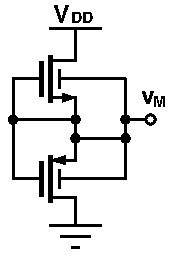
\includegraphics[width=0.2\textwidth, angle=0]{./figs/design/inv_vm}
			    \caption{Circuit to extract self-biased common mode level.}
			    \label{fig:inv_vm}
			\end{figure}

			\begin{figure}[htb!]
			    \centering
			    \begin{subfigure}{0.5\textwidth}
			        \centering
			        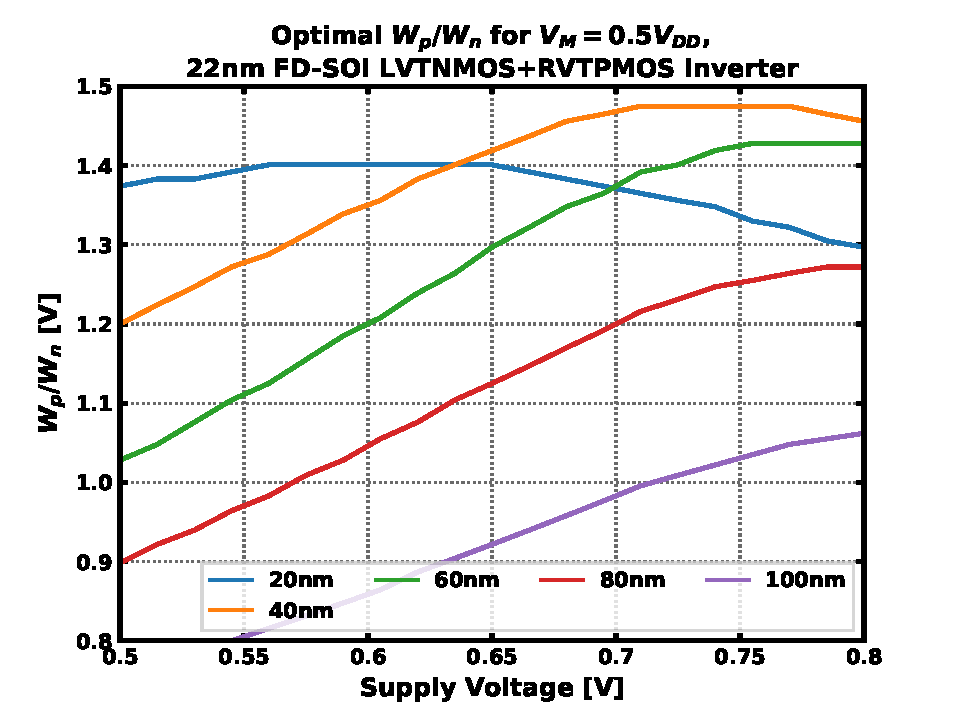
\includegraphics[width=1\textwidth, angle=0]{./figs/design/lvtnfet_pfet}
			        \caption{ }
			        \label{fig:ratio_lvtn_p}
			    \end{subfigure}%
			    \begin{subfigure}{0.5\textwidth}
			        \centering
			        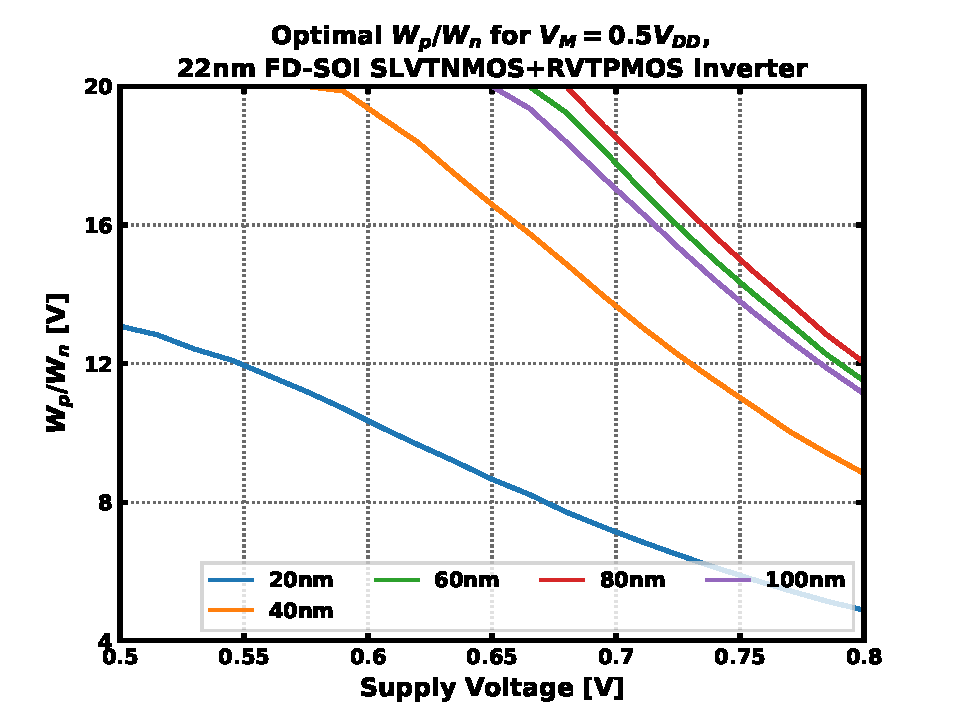
\includegraphics[width=1\textwidth, angle=0]{./figs/design/slvtnfet_pfet}
			        \caption{ }
			        \label{fig:ratio_slvtn_p}
			    \end{subfigure}
			    % \caption{x.}
			    \caption{\textbf{(a)} Optimal width ratio of RVTPMOS/LVTNMOS, \textbf{(b)} Optimal width ratio of RVTPMOS/SLVTNMOS.}
			    \label{fig:opt_ratio}
			\end{figure} 


	% \section{Estimating PSD with Autoregressive Model}\label{yule_walker_ar_psd}
	% The following is based on \cite{proakis_1993_psd}. Given a signal x[n] whose power spectrum should be estimated, its autocorrelation sequence $r_{xx}[l]$ with lag $l$ must be computed:
	% \begin{equation}
	% 	r_{xx}[l] = \sum_{n=-\infty}^{\infty} x[n]x[n-l]
	% \end{equation}
	% The autoregressive model for power spectrum, with p poles, that shall be fitted is given in \ref{eq:ar_psd_eq}
	% \begin{equation}\label{eq:ar_psd_eq}
	% 	S_{XX}(f) = \left.\frac{1}{|1+\sum_{n=1}^pa_nz^{-1}|^2}\right|_{z^{-1}=e^{-j2\pi f\Delta T}}
	% \end{equation}
	% MMSE optimization of the distribution for coefficients $\{a_1, ..., a_p\}$ is done by solving the Yule-Walker equation in \ref{eq:yule_walker}.
	% \begin{equation} \label{eq:yule_walker}
	% \begin{bmatrix}
	% a_1\\ 
	% a_2\\
	% \vdots\\
	% a_p
	% \end{bmatrix} = 
	% -\mathbf{R}_{xx}^{-1}\mathbf{r}_{xx}=
	% -\begin{bmatrix}
	% r_{xx}[0] & r_{xx}[1] & \dots & r_{xx}[p-1]\\ 
	% r_{xx}[1] & r_{xx}[0] & \dots & r_{xx}[p-2]\\ 
	% \vdots & \vdots &  & \\
	% r_{xx}[p-1] & r_{xx}[p-2] &  & r_{xx}[0]
	% \end{bmatrix}^{-1}
	% \begin{bmatrix}
	% r_{xx}[1]\\ 
	% r_{xx}[2]\\
	% \vdots\\
	% r_{xx}[p]
	% \end{bmatrix}
	% \end{equation}

% \vspace{-0.8em}\center$ \square $
	% \section{Oscillator phase noise due to thermal noise}\label{osc_pn_additive_append}


	% \begin{figure}[htb!]
	% 	\center\fontfamily{\sfdefault}\selectfont
% XCircuit output "dco_noise.tex" for LaTeX input from dco_noise.ps
\def\putbox#1#2#3#4{\makebox[0.00000in][l]{\makebox[#1][l]{}\raisebox{\baselineskip}[0.00000in][0.00000in]{\raisebox{#2}[0.00000in][0.00000in]{\scalebox{#3}{#4}}}}}
\def\rightbox#1{\makebox[0.00000in][r]{#1}}
\def\centbox#1{\makebox[0.00000in]{#1}}
\def\topbox#1{\raisebox{-0.60\baselineskip}[0.00000in][0.00000in]{#1}}
\def\midbox#1{\raisebox{-0.20\baselineskip}[0.00000in][0.00000in]{#1}}
   \scalebox{1}{
   \normalsize
   \parbox{3.56562in}{
   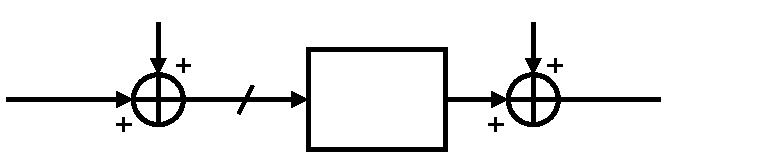
\includegraphics[scale=0.70000]{./figs/dco_noise.pdf}\\
   % translate x=-384 y=320 scale 0.38
   \putbox{1.02900in}{0.39200in}{0.96}{u[n]}%
   \putbox{1.48400in}{0.24500in}{0.96}{$\frac{2\pi K_{DCO}T}{1-z^{-1}}$}%
   \putbox{2.66700in}{0.34300in}{0.96}{$\Phi_{out}$[n]}%
   \putbox{0.78400in}{0.60900in}{0.96}{q$_{OTW}$[n]}%
   \putbox{0.18200in}{0.37800in}{0.96}{$\hat{\textnormal{u}}$[n]}%
   \putbox{2.54800in}{0.62300in}{0.96}{$\Phi_{n_{DCO}}$[n]}%
   } % close 'parbox'
   } % close 'scalebox'
   \vspace{-\baselineskip} % this is not necessary, but looks better
\fontfamily{\rmdefault}\selectfont

	% 	\caption{DCO additive noise model.}
	% 	\label{fig:dco_noise2}
	% \end{figure}
	% \FloatBarrier

	%  Oscillator phase noise due to stochastic and uncorrelated circuit and supply noise can be analyzed as additive voltage disturbance $\delta v_n$ with variance $\sigma_{v_n}^2$ to the oscillator waveform $V_{osc}$ at any given time.  In a stable, noiseless oscillator, amplitude is inherently tied to signal phase, i.e. $V_{osc}(\Phi=\omega t)$. With additive noise, given $\frac{dV_{osc}(\Phi)}{d\Phi}$ is finite $\forall$t, a small voltage disturbance from noise $\delta v_{n}$ will be coupled as a disturbance $\delta\Phi_{n}$ in the oscillator phase, shown in figure \ref{fig:aperture_noise}. The phase evolution of the noisy oscillator for an infinitesimal time increment $\delta t$  with such a disturbance is:
	%  \begin{equation}
	% 	\Phi_{out}(t+\delta t) = \Phi_{out}(t) + \delta\Phi_n + \omega_{osc}\delta t \label{eq:rwalk_ph}
	%  \end{equation}

	% \begin{figure}[htb!]
	% 	\center\fontfamily{\sfdefault}\selectfont
% XCircuit output "aperture_noise.tex" for LaTeX input from aperture_noise.ps
\def\putbox#1#2#3#4{\makebox[0.00000in][l]{\makebox[#1][l]{}\raisebox{\baselineskip}[0.00000in][0.00000in]{\raisebox{#2}[0.00000in][0.00000in]{\scalebox{#3}{#4}}}}}
\def\rightbox#1{\makebox[0.00000in][r]{#1}}
\def\centbox#1{\makebox[0.00000in]{#1}}
\def\topbox#1{\raisebox{-0.60\baselineskip}[0.00000in][0.00000in]{#1}}
\def\midbox#1{\raisebox{-0.20\baselineskip}[0.00000in][0.00000in]{#1}}
   \scalebox{1}{
   \normalsize
   \parbox{4.06875in}{
   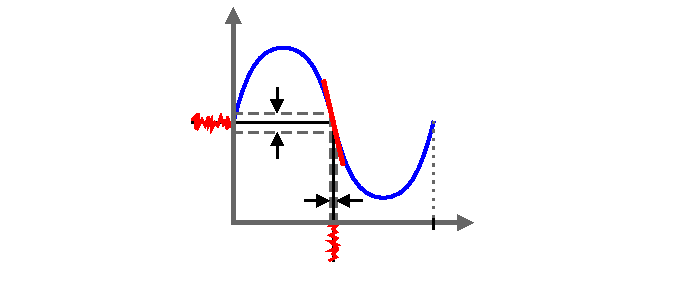
\includegraphics[scale=0.90000]{./figs/aperture_noise.pdf}\\
   % translate x=96 y=256 scale 0.38
   \putbox{2.82600in}{0.23400in}{0.96}{\rotatebox{-360}{$\Phi$}}%
   \putbox{1.19700in}{1.47600in}{0.96}{V}%
   \putbox{1.58400in}{1.21500in}{0.96}{$\sigma_{v_n}$}%
   \putbox{1.56600in}{0.48600in}{0.96}{$\sigma_{\Phi_n}$}%
   \putbox{1.00800in}{1.13400in}{0.60}{Thermal }%
   \putbox{1.08000in}{1.04400in}{0.60}{noise}%
   \putbox{1.66500in}{0.21600in}{0.60}{Phase }%
   \putbox{1.68300in}{0.12600in}{0.60}{noise}%
   \putbox{2.54700in}{0.21600in}{0.60}{\rotatebox{-360}{$2\pi$}}%
   \putbox{1.35900in}{0.21600in}{0.60}{$0$}%
   \putbox{0.90900in}{0.93600in}{0.96}{$\delta_{v_n}$}%
   \putbox{2.06100in}{0.09000in}{0.96}{$\delta_{\Phi_n}$}%
   \putbox{2.03400in}{0.90900in}{0.96}{$\frac{dV_{osc}(\Phi)}{d\Phi}$}%
   \putbox{1.62900in}{1.45800in}{0.60}{\rotatebox{-360}{$V_{osc}$}}%
   } % close 'parbox'
   } % close 'scalebox'
   \vspace{-\baselineskip} % this is not necessary, but looks better
\fontfamily{\rmdefault}\selectfont

	% 	\caption{Voltage to phase noise conversion.}
	% 	\label{fig:aperture_noise}
	% \end{figure}
	% \FloatBarrier
	%   Assuming $\delta v_n$ is Gaussian white noise, $\delta\Phi_{n}$ is sampled stochastically at any instant based on the probability distribution \ref{eq:osc_rw_dist}, dependent on the current oscillator phase $\Phi_{out}$ and the noiseless voltage-phase relation $V_{osc}(\Phi)$. It will be assumed that like the source noise $\delta v_n$, $\delta\Phi_{n}$ is white spectrum.
	%  \begin{equation}
	%  	P(\delta\Phi_{n}|\Phi_{out}) = \text{Norm}\left(\mu=0, \sigma=\sigma_{v_n}\left(\left.\frac{dV_{osc}(\Phi)}{d\Phi}\right\vert_{\Phi=\Phi_{out}}\right)^{-1}\right) \label{eq:osc_rw_dist}
	%  \end{equation} 
	% Spectral analysis of the noisy oscillator phase can be made utilizing discrete time-modeling. Converting \ref{eq:rwalk_ph} into a sampled signal with time step $\delta t$ 
	% \begin{equation}
	% 	\Phi_{out}[n+1] = \Phi_{out}[n] + \omega_{osc}\delta t + \delta\Phi_n[n|\Phi_{out}[n]]
	% \end{equation}
	% Computing the z-transform, and splitting the result into the oscillation $\Phi_{osc}$ and phase noise $\Phi_{n}$ components:
	% \begin{equation}
	% 	\Phi_{out}(z) = \frac{\omega_{osc}\delta t}{z-1} + \frac{\delta\Phi_n(z)}{z-1} = \Phi_{osc}(z) + \Phi_{n}(z)
	% \end{equation}
	% \begin{equation}
	% 	\Rightarrow \Phi_{n}(z) = \frac{\delta\Phi_n(z)}{z-1} \label{eq:z_osc_pn}
	% \end{equation}
	% Application of the bilinear transform to \ref{eq:z_osc_pn} can be used to approximate the continuous phase noise spectrum, if $s=j\omega$
	% \begin{equation}
	% 	\Phi_{n}(s) = \left.\Phi_{n}(z)\right\vert_{z=1-s\delta t} = \left.\frac{\delta\Phi_n(z)}{z-1}\right\vert_{z=1+s\delta t} = \frac{\delta\Phi_n(s)}{s\delta t}
	% \end{equation}
	% The phase noise PSD is therefore:
	% \begin{equation}
	% 	S_{\Phi n_{DCO}}(f)= \lim_{\Delta T\rightarrow\infty}\frac{1}{\Delta T}\left|\frac{\delta\Phi_n(j2\pi f)}{j2\pi f \delta t}*\mathcal{F}\left\{\text{rect}\left(\frac{t}{\Delta t}\right)\right\}\right|^2  =  \frac{S_{0\Phi n_{DCO}}}{f^2}
	% \end{equation}
	% Following that the phase disturbance signal $\delta\Phi_{n}(t)$ is white spectrum, a constant value for its PSD $S_{0\Phi n_{DCO}}$ can be defined. The value for $S_{0\Phi n_{DCO}}$ is highly dependent on implementation and is best extracted by means of curve fitting simulation or physical measurement.
